\selectlanguage{english}
\begin{abstract}
    \noindent A \emph{Számítógépes szimulációk} laboratórium második alkalmával az ingamodellek differenciálegyenleteinek numerikus megoldásait vizsgáltuk különböző közelítésekben (matematikai, csillapított, gerjesztett és fizikai). Összehasonlítottuk az egyenleteket megoldó negyedrendű Runge--Kutta, a lépéshossz-váltó (adaptív) negyedrendű Runge--Kutta, a Runge--Kutta--Cash--Karp és az adatív Runge--Kutta--Cash--Karp, valamint az Euler és az Euler--Cromer módszereket. Kiegészítésként megvizsgáltuk ezek pontosságát és érzékenységét a kettős ingára vonatkozóan is. \\
\end{abstract}
\selectlanguage{magyar}

\begin{multicols}{2}

\section{Feladatok} \label{sec:1}
A laboratórium második feladatában az ingák mozgásegyenleteinek numerikus közelítésével foglalkoztunk. A feladatok magukba foglalták mind az egyszerű matematikai, mind a gerjesztett-csillapított, mind pedig a fizikai ingák egyenleteivel történő munkát is. \\
A fentiek megoldásához néhány ismert differenciálegyenlet megoldó algoritmust kellett alkalmaznunk, amik eredményeit több szempont alapján is összevetettük egymással. A szóban forgó algoritmusok között a már első feladatból is ismert Euler- és Euler--Cromer-módszer foglalt helyet, valamint újdonságként a negyedrendú Runge-Kutta (innentől RK4) és a Cash-Karp (innentől RKCK) módszerek is szerepeltek a többi mellett. Az utóbbi kettő módszer esetében egy adaptív lépéshossz-változtató metódus is implementálva volt. Vizsgálataink arra irányultak, hogy az egyenlet megoldó algoritmusok melyik módszer esetében hogyan viselkednek, valamint, hogy azok pontosan mikre érzékenyek. Ehhez monitoroznunk kellett az ingák kitérését, sebességét és kinetikus energiájuk változását az idő függvényében minden módszer esetében. \\
Kiegészítésként implementálnunk kellett a kettős inga mozgásegyenleteit is, amiket szintén a fenti vizsgálatok alá volt szükséges vetnünk. \\
Megjegyzendő, hogy minden esetben az olyan mozgásokat vizsgáltuk, ahol minden ingát egy merev rúd rögzít a falhoz, vagy a kettős ingánál esetlegesen a másik ingához.

\section{Elméleti alapok} \label{sec:2}
A bonyolultabb klasszikus mechanikai rendszerek mozgásegyenletei legegyszerűbben az azokat leíró ún. \emph{Lagrange-függvény} által definiált funkcionálok variációs problémájának megoldásával - az adott funkcionál stacionárius pontjainak keresésével - kaphatóak. Ezek a pontok az ún. Euler--Lagrange-egyenlet megoldásával kaphatóak, mely maga a rendszer mozgásegyenlete lesz\cite{gyorgyigeza}. Ez a klasszikus mechanika egyik alapvető formalizmusa, így részletezésébe itt nem megyek bele. Míg az matematikai inga leírásához, annak egyszerűségéből kifolyólag ez a megközelítés értelmetlenül bonyolultabb a naiv felírásnál, addig a kettős ingához már elengedhetetlen eszközzé válik.

\subsection{Matematikai inga} \label{sub:2.1}
A gerjesztett-csillapított matematikai inga mozgásegyenlete célszerűen levezethető - pontos megfogalmazás szerint átalakítható -, ha Newton II. törvényét felírva átváltjuk a benne szereplő mennyiségeket polárkoordinátákba. A kiinduló egyenletünk ekkor az ismert

\begin{equation}
    \boldsymbol{F} = m \boldsymbol{a}
\end{equation}
amit az inga esetében felírhatunk a kitérés szöge és a kötél hosszának függvényében:

\begin{equation}
    \boldsymbol{F} = -m \boldsymbol{g} * \sin{\left( \theta \right)}
\end{equation}
Ezt leosztva $m$-el kapjuk a következő alakot:

\begin{equation}
    \boldsymbol{a} = -\boldsymbol{g} * \sin{\left( \theta \right)}
\end{equation}
A polárkoordinátákra történő átváltáshoz definiáljuk azt az ívhosszt, amit az inga leír. Ha ezt $k$-val jelöljük, akkor felírhatjuk az inga függőlegeshez viszonyított $\theta$ kitérési szögének függvényében:

\begin{equation}
    k = l * \theta
\end{equation}
ahol kis $l$ az inga kötelének (rúdjának) hossza. A kerületi sebeség ennek idő szerinti deriváltja:

\begin{equation}
    \frac{d k}{dt} = l * \frac{d \theta}{dt}
\end{equation}
Ennek újabb idő szerinti deriváltja pedig a gyorsulás, aminek értékébe a fent kapott eredményt be tudjuk helyettesíteni:

\begin{equation}
    \frac{d \left(l * \frac{d \theta}{dt} \right)}{dt}
    =
    l * \frac{d^{2} \theta}{dt^{2}}
    =
    -g * \sin{\left( \theta \right)}
\end{equation}
Ebből pedig a végleges mozgásegyenlet:

\begin{equation}
    \boxed{
    \frac{d^{2} \theta}{dt^{2}}
    =
    - \frac{g}{l} * \sin{\left( \theta \right)}
    }
\end{equation}

\subsection{Kettős inga} \label{sub:2.2}
A kettős inga mozgásegyenletének levezetéséhez fel kell írnunk a rendszer Lagrange-függvényét. Ennek segítségével a mozgásegyenlet kifejezhető a már említett variációs módszer és az Euler--Lagrange-egyenlet kifejtésének segítségével. Ennek levezetése hosszú, így azt és a végleges mozgásegyenleteket az \q{A} függelékben csatolom.

\section{Megvalósítás} \label{sec:3}
Előzetesen az egyszerű, gerjesztett-csillapított matematikai inga mozgásegyenletét megoldó, \texttt{C++} nyelven írt keretrendszer volt számunkra megadva, melyet a kitűzött feladatok alapján nekünk kellett bővítenünk. \\
A forráskódot az első feladathoz hasonlóan egy saját batch file segítségével, benne a \texttt{clang} fordító felhasználásával fordítottam. Az eredeti kód módosításával elértem, hogy a lefordított \texttt{exe} program egy Jupyter Notebook-ban futó Python 3 kernel segítségével induljon. A szimuláció a kezdőfeltételeket szintén ebből a környezetből várja, bemenő paraméterek formájában. \\
A szimpla- és a kettős inga két különböző \texttt{main} forrásfile alapján fordul. Az előbbi outputja egy, míg utóbbi esetében két különböző \texttt{.dat} file. A különbség, hogy míg a szimpla inga esetében csak az inga aktuális kitérése, sebessége, valamint kinetikus energiája van az outputban monitorozva, addig a kettős ingánál egy külön adatfile szolgál a két inga aktuális x-y koordinátáinak tárolására. \\
Opcionális lehetőség volt, hogy egy előre megírt \texttt{C++} OpenGL környezetet használjunk a mozgások ábrázolására, azonban esztétikai okokra hivatkozva ehelyett ezt Pythonban valósítottam meg egy saját kód segítségével. Ez a \texttt{matplotlib} és a \texttt{imageio} könytárakat használva generál megadott paraméterek alapján \texttt{mp4} formátumú, kis méretű, de nagy felbontású videókat az ingák mozgásáról. \\
A végleges forráskód és a programot futtató Notebook file-ok elérhetőek GitHub-on\cite{github}.

\section{Kiértékelés} \label{sec:4}
\subsection{A matematikai inga mozgása} \label{sub:4.1}
Az előzetesen megadott kódban szereplő gerjesztett-csillapított ingát több esetre is megvizsgáltam, ezek az alábbiak voltak:
\begin{enumerate}
    \item Gerjesztés és csillapítás nélküli eset
    \item Kizárólag csillapított mozgás
    \item Egyszerre csillapított és gerjesztett eset
    \item Kizárólag gerjesztett mozgás
\end{enumerate}
Ezek mindegyikét, azonos paraméterekkel futtattam a (\ref{sec:1})-es pontban felsorolt differenciákegyenlet megoldó algoritmusokon, és minden futtatás esetében felvettem a rendszer idő-kitérés és idő-sebesség, valamint a kitérés-sebesség és sebesség-energia grafikonját, 2-2 ábrára rendezve őket. Ilyen módon ez a 6 algoritmusra összesen 48 ábrát eredményezett. Ezeket a rendkívüli hosszuk miatt a \q{B} függelékben csatolom. A (\ref{fig:4}) - (\ref{fig:27}) ábrák (B.1. függelék) a szimpla ingára felvett kitérés-idő és sebesség idő grafikonok a különböző esetekre és iterációs módszerekre vonatkozóan. A (\ref{fig:28}) - (\ref{fig:51}) ábrák (B.2. függelék) az ezekhez tartozó fázis-, valamint energia-sebesség diagramok, az előzőekkel azonos sorrendben és elhelyezkedésben.
\\
A kezdeti feltételeket az ábrázoláshoz minden közelítés esetében - ahol természetesen a speciális feltételek ezt nem korlátozták - azonosan választottam meg. Ezt alább két táblázatban ismertetem:

\begin{center}
\begin{tabular}{c||c|c|c|c|c}
    \hline
    Paraméter & $t$     & $dt$     & $m$     & $l$    & $\theta_{0}$  \\ \hline
    Érték     & $30$ s  & $0.1$ s  & $1$ kg  & $1$ m  & $80^{\circ}$  \\ \hline
\end{tabular}
\end{center}
\captionof{table}{\normalfont A szimpla ingás szimulációk konstans kezdőfeltételei}\label{tab1}

\begin{center}
\begin{tabular}{c||c|c|c}
    \hline
    Paraméter    &  $q$   & $\Omega_{D}$  & $F_{D}$  \\ \hline\hline
    Mat.         & $0$    & $0^{\circ}$   & $0$ N    \\ \hline
    Damp.        & $0.4$  & $0^{\circ}$   & $0$ N    \\ \hline
    Damp.-Driv.  & $0.4$  & $30^{\circ}$  & $4$ N    \\ \hline
    Driv.        & $0$    & $30^{\circ}$  & $4$ N    \\ \hline
\end{tabular}
\end{center}
\captionof{table}{\normalfont A szimpla ingás szimulációk változó kezdőfeltételei}\label{tab2}
\hfill \break
Ahol az első táblázatban $t$ a szimulált idő, $dt$ pedig a lépésközök hosszát, $m$ az inga tömegét, $l$ az kötél hosszát, $\theta_{0}$ pedig az inga, függőlegeshez mért kezdeti kitérésének szögét jelöli. Hasonlóan a második táblázatban $q$ a rendszer csillapítási tényezőjét, $\Omega_{D}$ a gerjesztés frekvenciáját, $F_{D}$ pedig a gerjesztő erő nagyságát jelenti.
\\ \\
A (\ref{fig:4})-(\ref{fig:51}) ábrákon jól látható a különböző kezdőfeltételek és iteratív módszerek közti különbség. Míg az RKCK, RK4 és ezek adaptív változatai nem mutatnak szemmel látható eltérést, addig az Euler--Cromer-módszer pontatlansága könnyebben észlelhető rajtuk, míg az explicit Euler-módszer minden szempontból kilóg az eredmények közül. \\
Az utóbbi használatánál - ismerve annak metodikáját - azt várnánk, hogy az energia nem marad meg, folyamatosan növekszik. Ez látható a róla készült ábrák esetében is, ahol az inga kitérése és sebessége, és így a rendszer energiája időben folyamatosan nő. Az ábrákból egyértelműen megállapítható, hogy alkalmatlan módszer az ingamozgás szimulálására. \\
A matematikai inga esetében a fázisdiagram egy ellipszis, amit mind a négy különböző Runge--Kutta-módszer helyesen visszad. Az Euler--Cromer-módszer esetében azonban a várt ellipszis kissé torzult, \q{csavart}. Ez az iterációs módszer ismerten pontatlanabb, mint az előbb említett függvénycsalád, ami ezen a feladaton keresztül szemléltethető is. Ez a torzulás azonban a lépésköz csökkentésével javítható, $dt = 0.01\ s$ esetén ez a metódus is szemmel láthatólag tökéletes ellipszist ad eredményül (lásd a Notebook file-t GitHub-on\cite{github}). Ebből következtethetünk rá, hogy a módszer nem alkalmazható rossz felbontású szimulációk esetén, azonban jó választás lehet a többi esetben (ami majd az \ref{sub:4.4}-es pontban ismertetett futásideje miatt is igaz).

\subsection{A kettős inga mozgása} \label{sub:4.2}
A kettős inga mozgásegyenleteteit és az azokat megoldó iteratív algoritmusokat - a már meglevőkre építve, de - teljes egészében nekünk kellett implementálnunk. Ezt egy külön forrásfile-ban valósítottam meg, aminek keretét az akkor már a saját változtatásaimmal együtt elkészült szimpla inga forrásfile-jából kölcsönöztem. \\
A kettős inga mozgását azonban kizárólag az RKCK és az RK4 módszerek segítségével elemeztem. Az adaptív módszerek szimplán túl lassú futásidőt eredményeztek ebben az esetben, míg a szimuláció az Euler- és Euler--Cromer-módszerrel futtatva már $t \approx 1\ s$ esetén is elszállt. A többi ábra mellett teljesen értelmetlennek láttam egy olyan, maximum 3-4 lépésből álló szimulációt ábrázolni, amiben az 5-6. lépésnél az energia már a $10^{18}$ nagyságrendnél tart. \\
Ennél a feladatnál már nem csak a szimpla ingánál ismertetett mennyiségeket vizsgáltam, hanem az ingák síkban történő mozgásának koordinátáinak változását is és egyéb effektusokat is. Ez összesen 52 db ábrát eredményezett, amiket az első feladathoz hasonlóan, a jelentős darabszámuk miatt a \q{B} függelékben csatoltam. \\
Az ábrák többek között a \ref{sub:4.1}-ben olvasottakhoz hasonlóan helyezkednek el a B.3-as és B.4-es függelékben. A (\ref{fig:52}) - (\ref{fig:59}) ábrák az RK4 és RKCK algoritmusokhoz tartozó kitérés-idő és sebesség-idő diagramok, amiket szintén a szimpla ingához hasonlóan, matematikai, csillapított, gerjesztett és csillapított, valamint csak gerjesztett esetekben vizsgáltam. A (\ref{fig:60}) - (\ref{fig:63}) ugyanezen diagramok összehasonlítása látható. Az egyetlen különbség (\ref{fig:52}) - (\ref{fig:59})-hoz képest, hogy itt egy ábrán vettem fel mind az RKCK, mind pedig az RK4-ből kapott kitérés értékeket az idő függvényében. Habár mindkét szimuláció teljesen azonos kezdőfeltételekkel indult, mégis erőteljes eltérés van a kettő között. Ez annak tudható be, hogy az RKCK és az RK4 algoritmusok nem teljesen azonosak, egymáshoz képest nagyon apró, de mégis eltérő numerikus hibákat produkálnak. Mivel a kettős inga egy kaotikus rendszer, így az apró, de különböző perturbációk is teljesen más és más kimeneteket képesek okozni az egyes esetekben. Pontosan ez látható ezeken az ábrákon is. \\
A B.4-es függelékben (\ref{fig:64}) - (\ref{fig:87}) értelemszerűen a fenteikhez tartozó fázisdiagramok és energia-sebesség grafikonok találhatóak. \\
A B.5-ös függelékben a kettős ingák által leírt trajektóriákat ábrázoltam (\ref{fig:88}) - (\ref{fig:95})-ig. Az ingamozgás síkban történik, így ezek ábrázolásához is csupán két koordinátát kellett figyelembe vegyek. Ezek felvételéhez az ingák felfüggesztését vettem egy Descartes-koordinátarendszer origójának, aminek segítségével az ingák kitérése és a rudak hossza alapján megkaptam az adott pillanatnyi pozíciókat. Az ábrákon külön ábrázoltam a két ingát minden esetben. Ez rajtuk egyértelműen jelölve is van. \\
A B.6-os függelékben az kettős inga kaotikus viselkedését használtam. Erről már az előbb említést tettem, ott azonban a különböző numerikus megoldásokból fakadó eltérésekről beszéltem. A (\ref{fig:96}) - (\ref{fig:103}) képeken azt vizsgáltam, hogy a kezdeti kitérítési szöget a 4-5. tizedesjegyben perturbálva, milyen hatással van ez a további mozgásra. Az ábrákon szépen látszik is az elvárt viselkedés: A legapróbb eltérések is teljesen különböző kimenetet produkálnak. Az ábrázolt 4 db kettős inga mozgása az eleján még együtt mozog, azonban egy pontban ezek hirtelen mind elválnak egymástól. Ez feltehetően egy olyan helyen következik be, ahol az iteratív módszerek viszonylag csak nagy hibával tudják a szimulációt léptetni. (Pl. ahol ott épp megfordul a sebességvektor iránya, így a gyorsulás egy hatalmas értékké nő.)

\subsection{Kettős inga - animáció} \label{sub:4.3}
A kettős ingához a Python \texttt{matplotlib} és \texttt{imageio} könyvtárainak felhasználásával egy olyan saját programot írtam, ami kimenetként képes animáció (pl. egy \texttt{mp4} kiterjesztésű videó) formájában ábrázolni egy tetszőleges paraméterekkel futtatott szimulációt. Erről több videót is készítettem, különböző bemenő paraméterekkel, amik közül néhány relevánsabbat a YouTube-on elérhetővé tettem, azok ott most is megtekinthetőek\cite{yt}.

\subsection{Futásidő} \label{sub:4.4}
A különböző iteratív módszerek futásidejét a matematikai inga esetére teszteltem. Az program futása alatt eltelt időt a \texttt{chrono} library segítségével mértem, milliszekundumos pontosságú időmérési metódust használva. A szimulációt a különöböző módszerekkel $t = 10\ s$ és $t = 120\ s$ közötti időpontokban futtattam a matematikai inga esetére, a fenti táblázatokban is szereplő kezdőfeltételekkel. Az egyes $t$ időkre történő futások között másodperces lépésekkel vettem fel a futásidőket. Ezeket az alábbi grafikonokon ábrázoltam:
\hfill \break \hfill \break
{\centering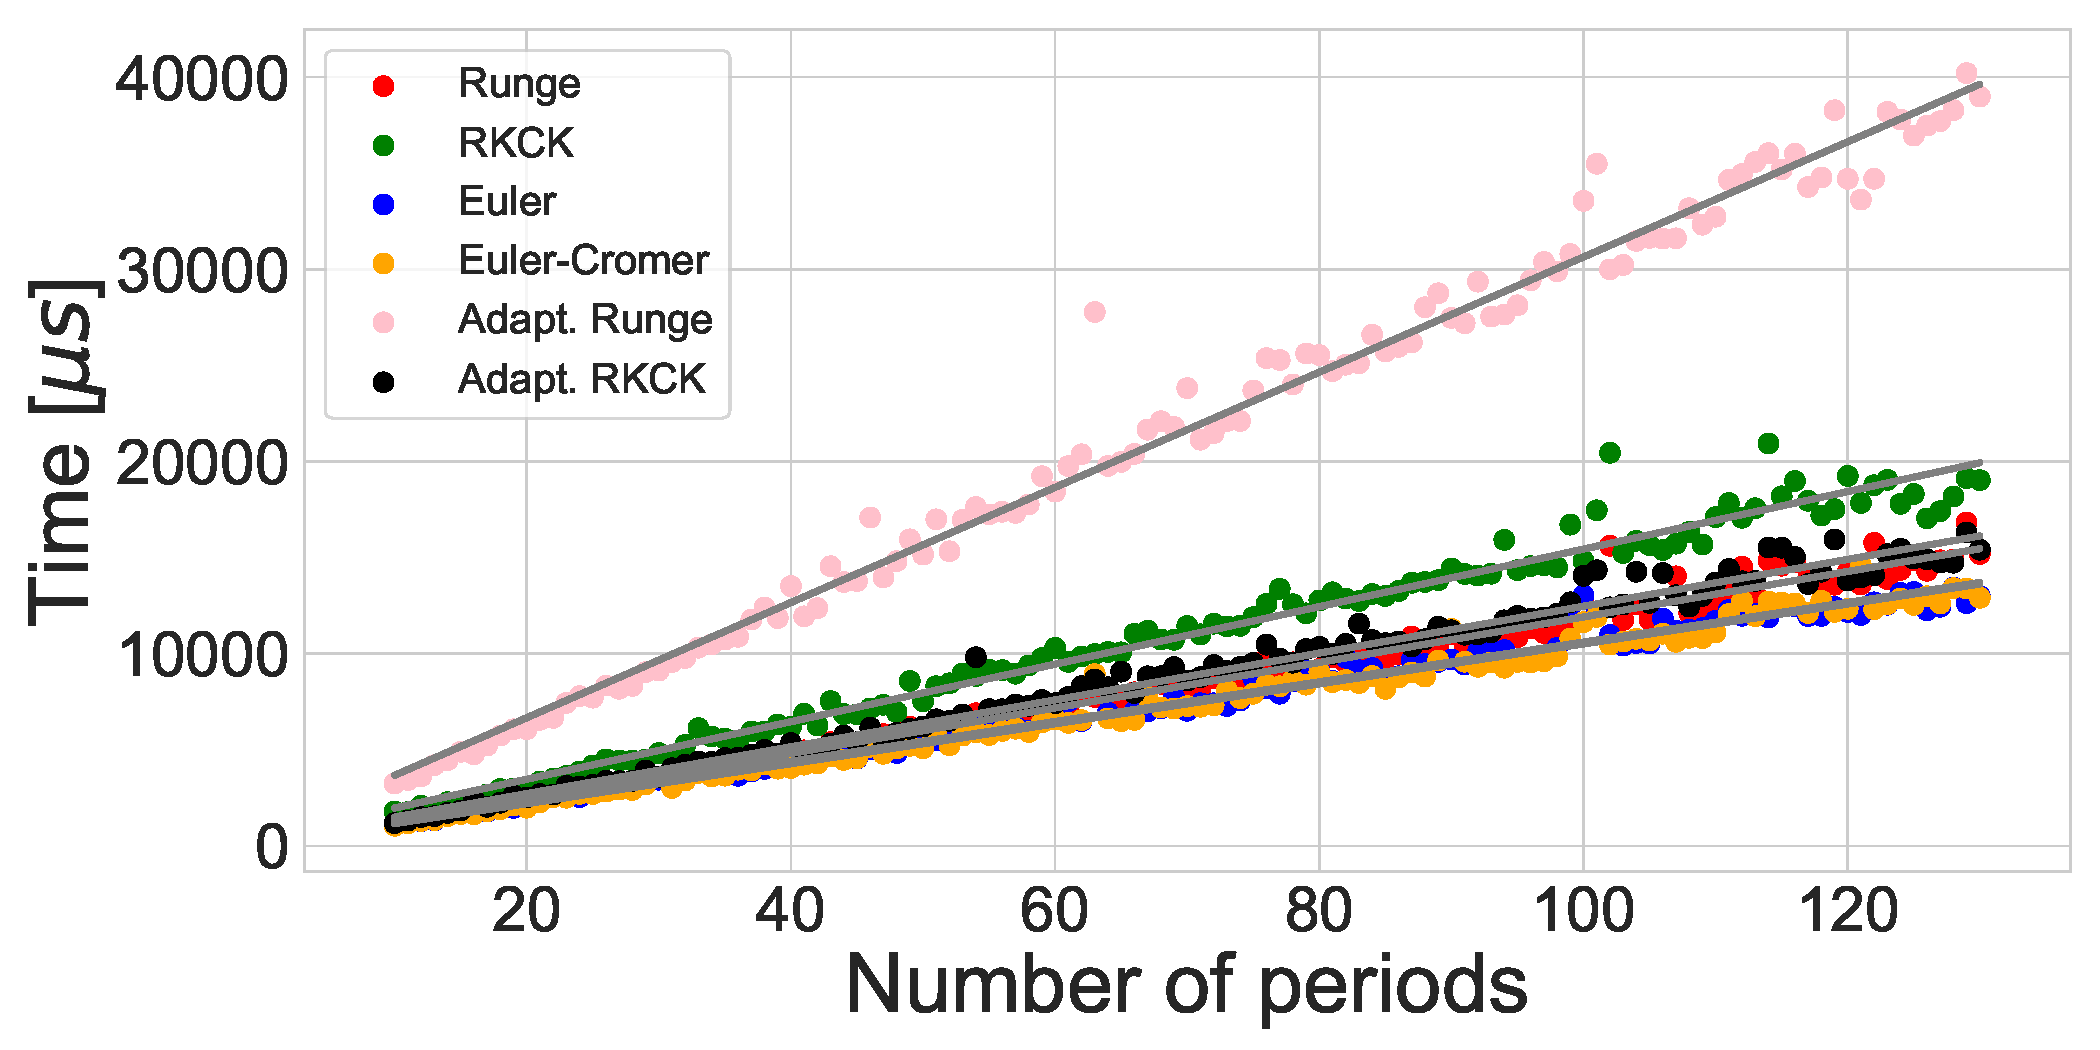
\includegraphics[width=.5\textwidth]{images/runtime_all.pdf}}
\captionof{figure}{Futásidők 1.\\Mat.}
\hfill \break
Az ábrán egyértelműen látszik, hogy az adaptív RK4 módszer magasan a leghosszabb futásidőt igénylő algoritmus. Hogy a többit jobban össze lehessen hasonlítani, a következő ábrából kihagytam az erre a módszerre kapottakat és csak a többit ábrázoltam:
\hfill \break \hfill \break
{\centering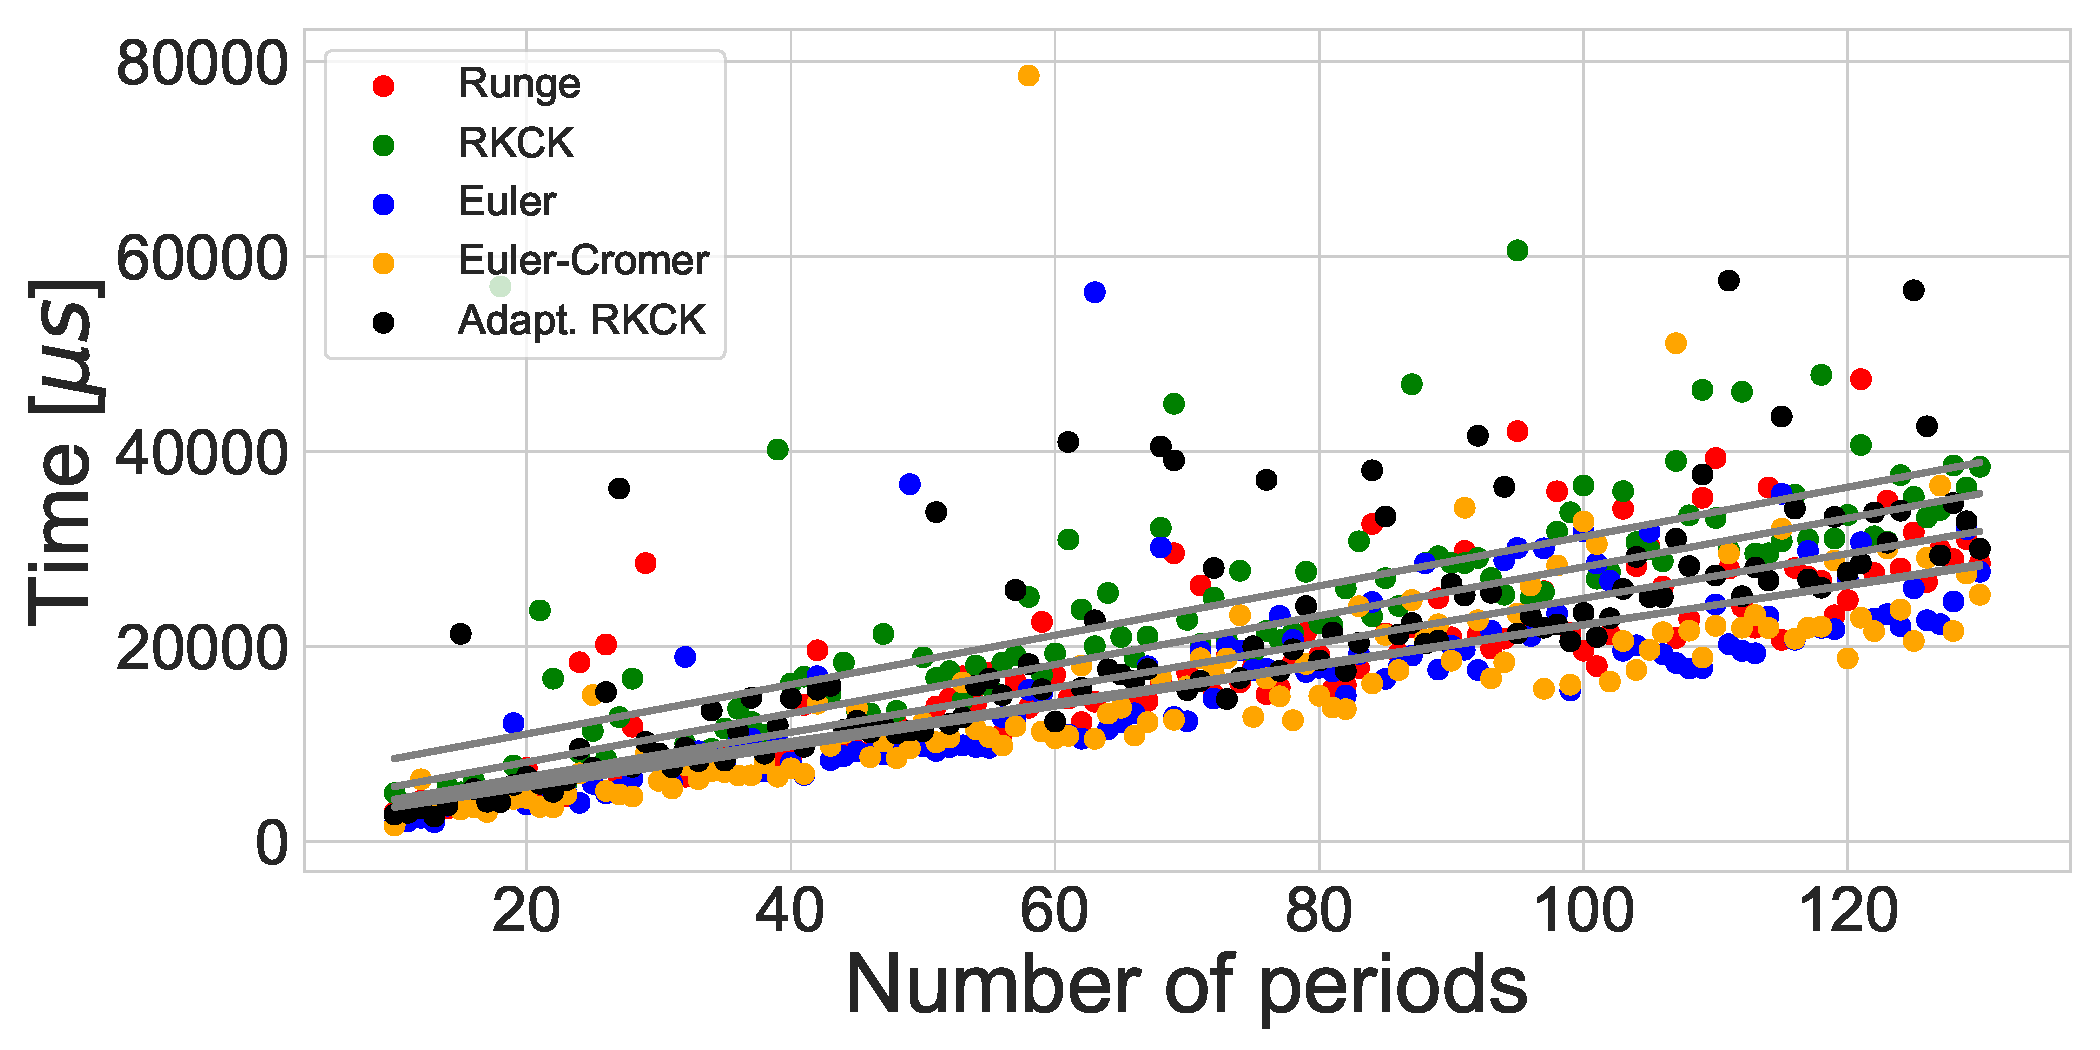
\includegraphics[width=.5\textwidth]{images/runtime_all_wo_runge.pdf}}
\captionof{figure}{Futásidők 2.\\Mat.}
\hfill \break
Már az előzőn is, de itt még szembetűnőbb, hogy az RKCK és annak adaptív variációja kilóg a többi közül. Ez nem csoda, hiszen jóval több, órajelet igénylő műveletet kell elvgeznünk közben, mint az összes többi maradék esetében. \\
Egyedül az Euler- és az Euler--Cromer-módszer esetén várnánk azonos futásidőt, hisz mindkettőben pontosan ugyanannyi és ugyanolyan műveletet végzünk el a szimuláció során - már ha a megírt algoritmusunk megfelelő. Ezt ellenőrizendő, ezt a kettőt is külön megvizsgáltam, amit az alábbi ábrán ismertetek:
\hfill \break \hfill \break
{\centering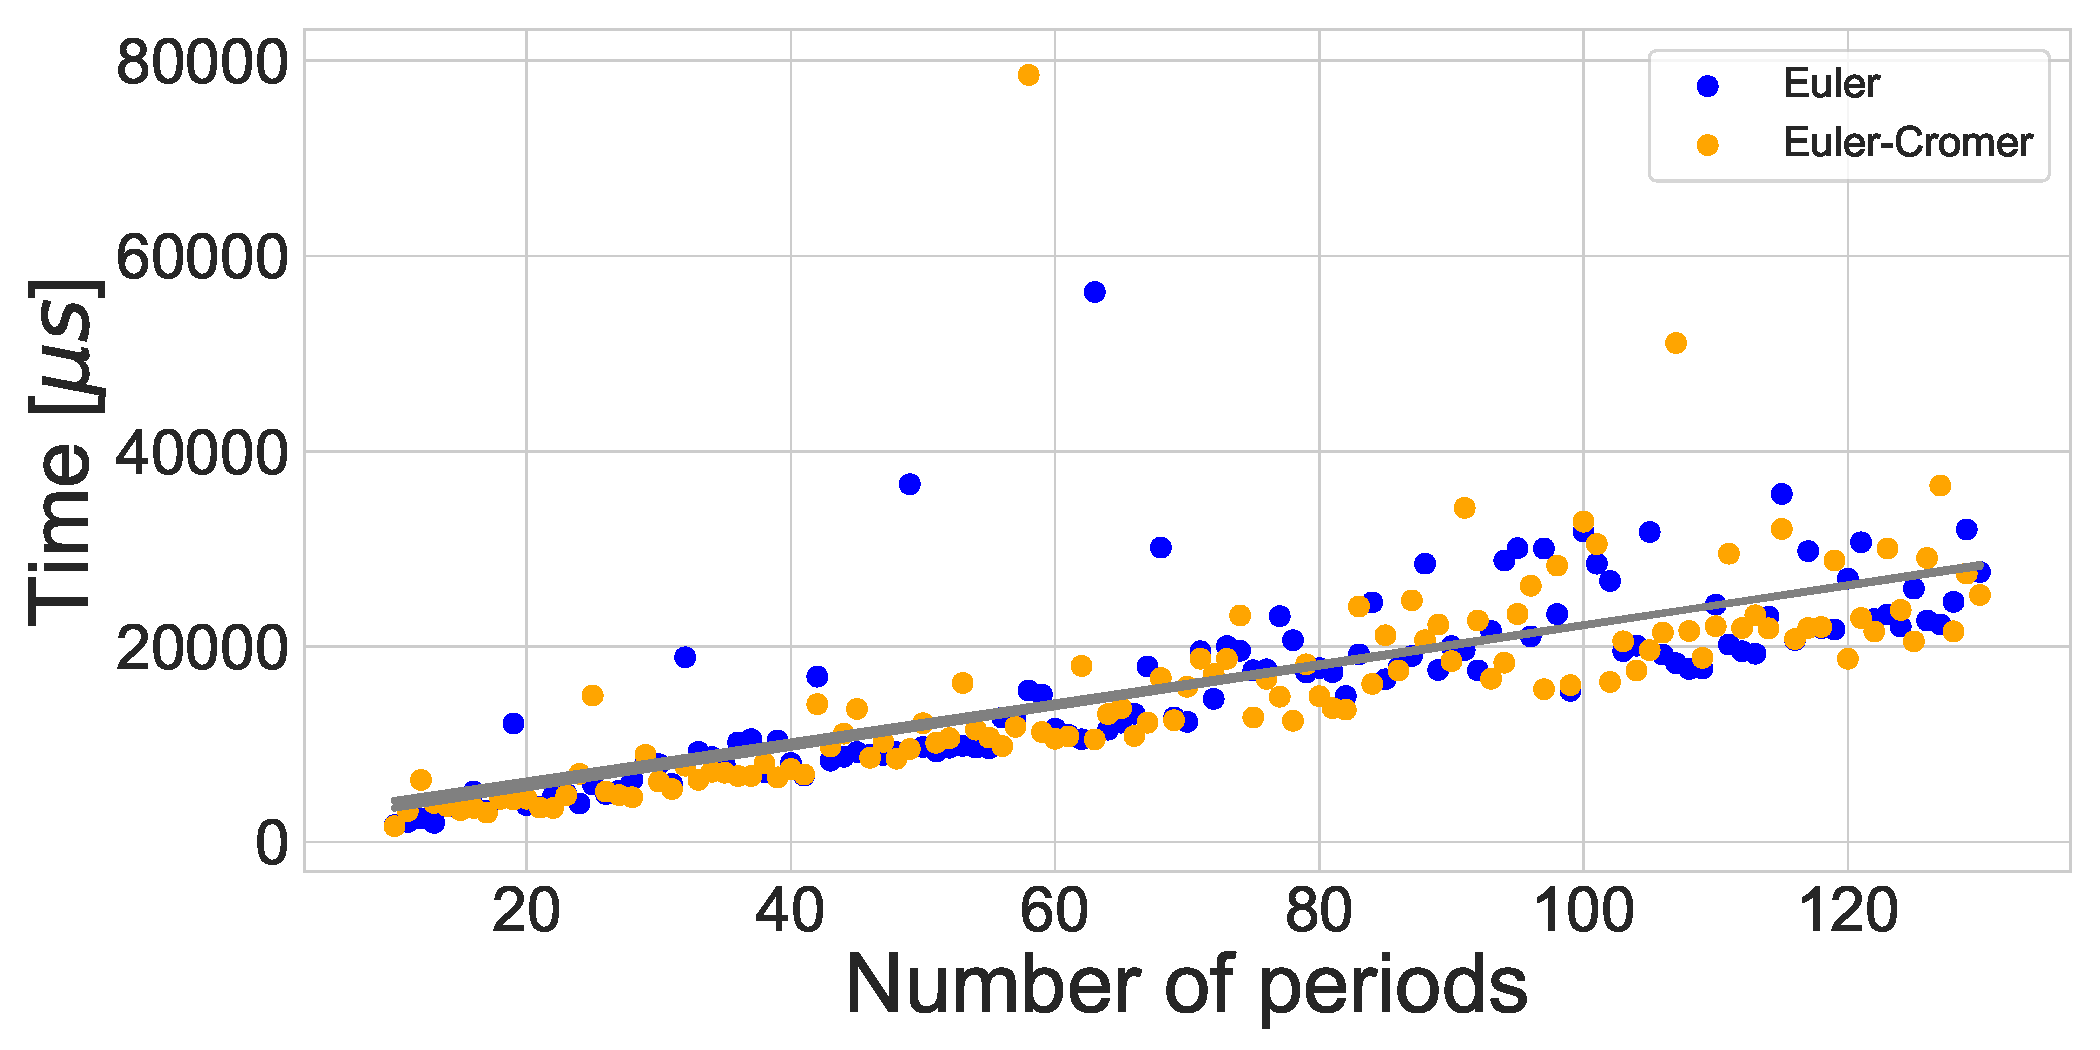
\includegraphics[width=.5\textwidth]{images/runtime_all_both.pdf}}
\captionof{figure}{Futásidők 3.\\Mat.}
\hfill \break
A kettő közti alig észrevehető különbség egyedül abból fakadhat, hogy az Euler--Cromer módszer esetén a biztonság kedvéért egy plusz értékadás műveletet is alkalmaztam, aminek szintén van - minimális, de véges nagyságú - órajeligénye. \\
Összefoglalóként azt mondhatjuk, hogy az Euler--Cromer-módszer minden esetben pontosabb képet ad az Euler módszernél, viszont futásidőben tökéletesen azonosak. Ellenben ebből a szempontból jobbak is a náluk pontosabb algoritmusoknál. Azt mondhatjuk tehát, hogy megfelelő rendszer szimulációjánál, kellően pontos lépésközt válaszva, érdemes lehet az Euler--Cromer-módszerhez folyamodni, ha a futásidő kulcsfontosságúan számít.

\section{Diszkusszió} \label{sec:5}
A feladatok során összehasonlítottam az ingamozgás példáján keresztül néhány ismert iteratív algoritmust, amik alkalmasak a fizikában előkerülő problémák numerikus közelítésére. Megállapítottam, hogy az Euler-módszer csak nagyon kivételes esetben érdemes alkalmazni, akkor is csak körültekintéssel, megfelelő szimulációs felbontás mellett. A vele megegyezően gyors futásidejű Euler--Cromer-módszer - habár még mindig nem pontosabb, mint a Runge--Kutta függvénycsalád - ellenben jó választásnak számíthat időigényes szimulációk optimalizációjához. \\



\section{Megjegyzések} \label{sec:6}
A dokumentumban található képek 150 dpi felbontású, \code{.pdf} kiterjesztésű forrásból származnak, amiket a \code{matplotlib} package \code{savefig} függvényének segítségével mentettem le. Ezek miatt a jegyzőkönyv néha lassan tölt be, azonban a már többször említett GitHub repository-ban az könnyebben olvasható. (Ennek az oka feltehetően az, hogy GitHub-on megnyitva az oldal az egész PDF-et betölti, míg egy offline PDF olvasó csak egy adott tartományban levő részeket az optimalizáció miatt.) \\

\end{multicols}